\begin{figure}[t]
  \centering
  \resizebox{\textwidth}{!}{%
    \begin{minipage}{\textwidth}
      \centering
      \begin{subfigure}[b]{0.22\textwidth}
        \centering
        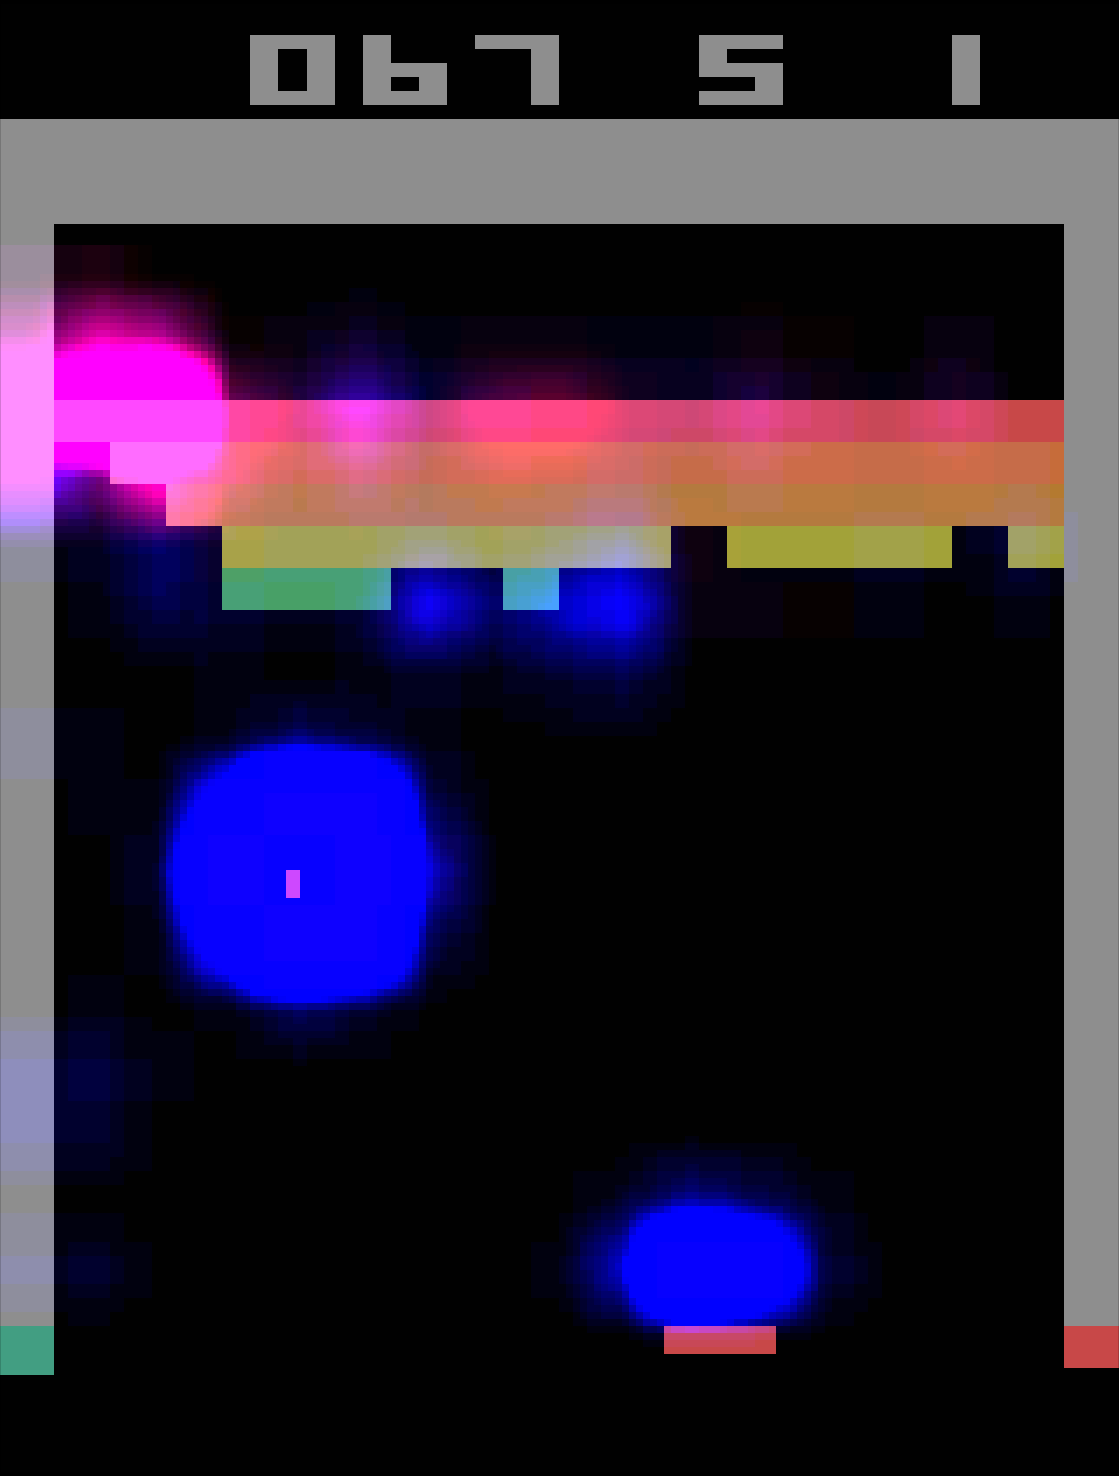
\includegraphics[width=0.5\linewidth]{figures/explainability_reinforcement_learning/hit_map.png}
        \caption{Perturbation-based heatmap for the Atari game ``Breakout'' \cite{greydanus2018visualizing}. Highlighted areas correspond to the most influential regions for the policy function's decision.}
        \label{fig:saliency_map_heatmap}
      \end{subfigure}
      \hfill
      \begin{subfigure}[b]{0.22\textwidth}
        \centering
        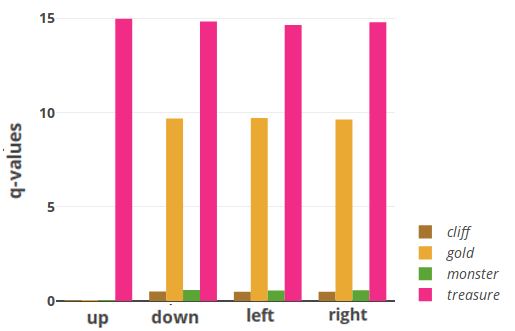
\includegraphics[width=\linewidth]{figures/explainability_reinforcement_learning/multi_q_values.png}
        \caption{Prediction of sub-rewards as a function of the action selected by the agent for a given state \cite{juozapaitis2019explainable}. Depending on the action chosen by the agent, one can determine which sub-reward it aims to maximize.}
        \label{fig:trajectory_prediction_values}
      \end{subfigure}
      \hfill
      \begin{subfigure}[b]{0.22\textwidth}
        \centering
        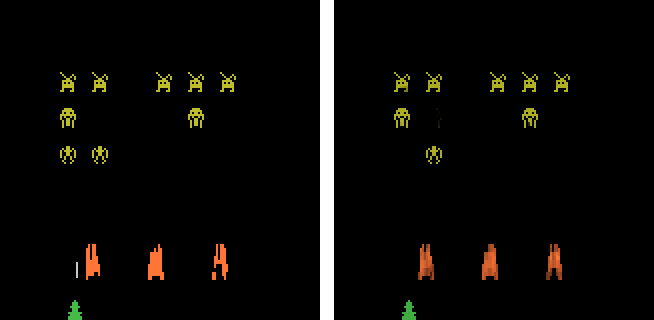
\includegraphics[width=\linewidth]{figures/explainability_reinforcement_learning/contrefactuel.png}
        \caption{Counterfactual explanation of the agent's behavior for the game \textit{Space Invaders} \cite{olson2021counterfactual}. In the left image, the observation leads to the action ``LEFT'', whereas in the right image, the action selected by the agent is ``RIGHT\_FIRE''.}
        \label{fig:counterfactual_example}
      \end{subfigure}
      \hfill
      \begin{subfigure}[b]{0.22\textwidth}
        \centering
        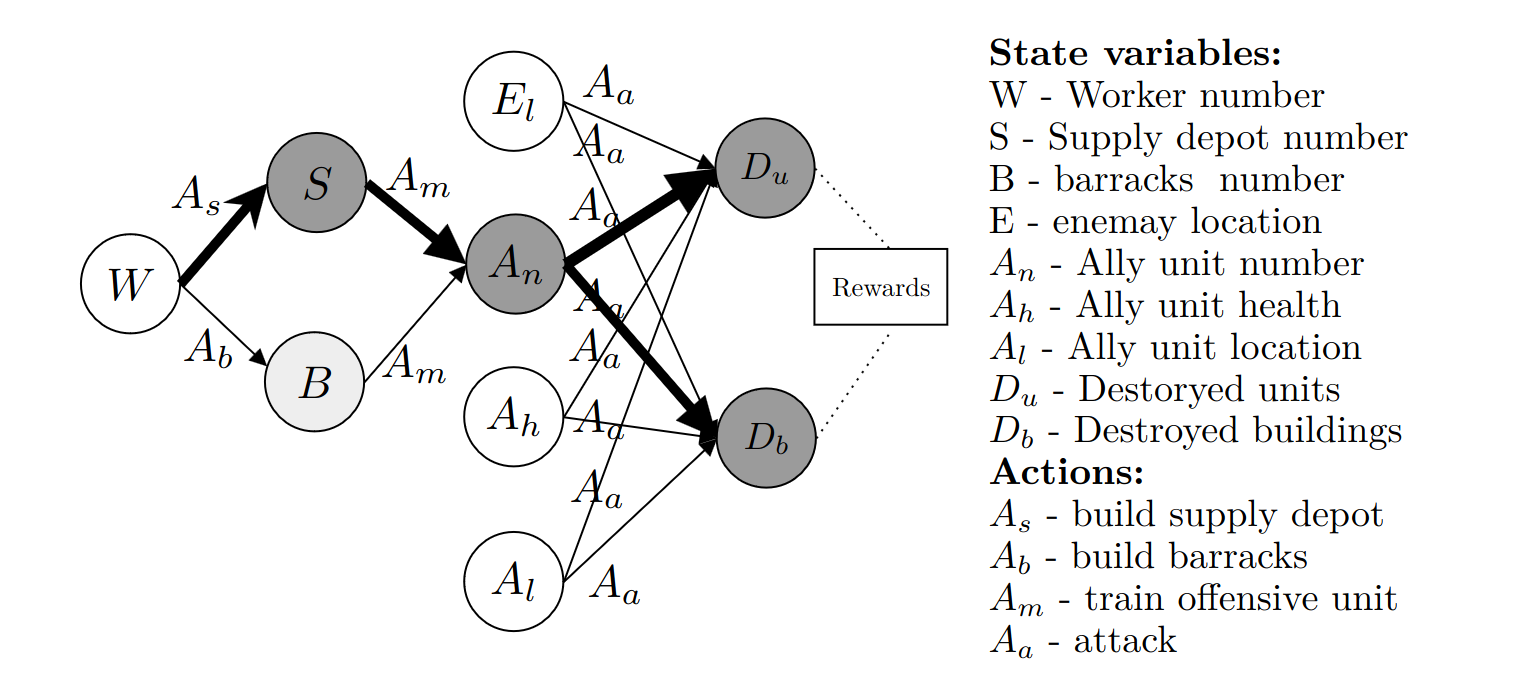
\includegraphics[width=\linewidth]{figures/explainability_reinforcement_learning/graph_causal.png}
        \caption{Agent--environment interaction model for the video game \textit{StarCraft II} \cite{madumal2020explainable}. Nodes represent random variables, and edges represent causal relationships between them.}
        \label{fig:interaction_model_causal_graph}
      \end{subfigure}
    \end{minipage}
  }
  \caption{Overview of XRL explanation methods. \textbf{(a)} Saliency map, \textbf{(b)} decomposed Q-values, \textbf{(c)} counterfactual states, \textbf{(d)} causal graph.}
  \label{fig:xrl_methods_overview}
\end{figure}
